\documentclass[10pt,a4paper]{article}

\usepackage[utf8]{inputenc}


\usepackage{algpseudocode}
\usepackage{algorithmicx}
\usepackage{amsfonts}
\usepackage{amsmath}
\usepackage{amssymb}
\usepackage[spanish]{babel}
\usepackage[style=nature,intitle=true,sorting=none]{biblatex}
\usepackage{csquotes}
\usepackage{dsfont}
\usepackage{enumitem}
\usepackage{fancyhdr}
\usepackage{geometry}
\usepackage{graphicx}
\usepackage[hidelinks]{hyperref}
\usepackage{ifthen}
\usepackage[utf8]{inputenc}
\usepackage{multicol}
\usepackage{titling}
\usepackage{xcolor}
\usepackage{wrapfig}


%%%% CONFIGURACIONES %%%%

%% La coma de los reales es un punto
\decimalpoint

%%% Tamaño de pagina
%\geometry{
%	includeheadfoot,
%	left=2.54cm,
%	bottom=1cm,
%	top=1cm,
%	right=2.54cm
%}

%\stul{0.1cm}{0.2ex}

%% HEADER Y FOOTER
\pagestyle{fancy}

\fancyhf{}

\fancyhead[LO]{\rightmark} % \thesection\ 
\fancyhead[RO]{\small{\thetitle}}
\fancyfoot[CO]{\thepage}
\renewcommand{\headrulewidth}{0.5pt}
\renewcommand{\footrulewidth}{0.5pt}
\setlength{\headsep}{1cm}
\setlength{\headheight}{13.07225pt}

\renewcommand{\baselinestretch}{1.2}  % line spacing

%% Links en indice 
\hypersetup{
	linktoc=all,     %set to all if you want both sections and subsections linked
	linkcolor=blue,  %choose some color if you want links to stand out
}

\newcommand{\red}[1]{{\color{red}#1}}
\newcommand{\nat}{\ensuremath{\mathbb{N}}} 					% Naturales
\newcommand{\reales}{\ensuremath{\mathbb{R}}} 				% Reales
\newcommand{\xDots}[2]{\ensuremath{#1_1,\dots, #1_{#2}}}


\newcommand{\dom}[1]{\text{dom}(#1)}

\newcommand{\comp}[4]{\ensuremath{#1(#3_1(\xDots{x}{n}),\dots,#3_#2(\xDots{x}{n}))}}
	
	
\newcommand{\resta}{\dot{-}}
\newcommand{\imagen}[4]{
\begin{figure}[ht]
	\centering
	\includegraphics[width=#1\textwidth]{#2}
	\caption{#3}
	\label{#4}
\end{figure}
}

\tikzstyle{demoBox} = [
draw=gray, very thick,
rectangle split, rectangle split parts=2, rounded corners, inner sep=2.5mm, inner ysep=2mm,
rectangle split part fill = {blue!40, blue!5}
]

\NewEnviron{demo}{%
\begin{center}
	\begin{tikzpicture}
	\node [demoBox](box){%
		\textbf{\scriptsize DEMOSTRACION}
		\nodepart{two}
		\begin{minipage}{0.85\textwidth}
		\BODY
		\begin{flushright}
		$\blacksquare$
		\end{flushright}
	
		\end{minipage}
	};
	\end{tikzpicture}
\end{center}
}
\title{Ingenieria I - Apuntes}

\begin{document}
	
\maketitle
\tableofcontents
\newpage
\section{Introduccion}
\paragraph{Sistemas reactivos:} Sistemas que reaccionan a estímulos provenientes de su entorno. Nos referimos a los estímulos y reacciones como \textbf{eventos} o \textbf{acciones}.


\subsection{Model Checking}
El \textbf{model checking} es una técnica para verificar sistemas concurrentes con estados finitos. El procedimiento, normalmente usa una búsqueda exhaustiva sobre el espacio de los estados del sistema para determinar si una especificación es correcta o no. Si se tienen los recursos suficientes (de harwdware), entonces siempre termina con una respuesta que puede ser \textbf{si} ó \textbf{no}. Además, puede ser implementada con algoritmos razonablamente eficientes que puede ser corridos en máquinas promedio. 

Aplicar la comprobación a un diseño consiste en varias tareas:

\paragraph{Modelado:} Convertir el diseño en un formalismo aceptado por la herramienta de comprobación (En nuestro caso el FSP). En muchos casos, esto es solo una compilación. En otros, debido a limitaciones de tiempo y memoria, puede requerir el uso de ciertas abstracciones para eliminar detalles irrelevantes al problema que tratamos de resolver.


\paragraph{Modelo:} Representación simplificada del mundo real que incluye solo aquellos aspectos del sistema que son relevantes al problema.

\paragraph{Proceso:} Ejecución de un programa secuencial de un programa. El estado de un proceso, en cualquier momento del tiempo, consiste en los valores de variables explicitas (declaradas por el programador) y variables implicitas (program counter, registros de direcciones, etc). 

Los modelos que vamos a usar ignora estos detalles de implementación y considera que un cambio de estado es producido por acciones  atómicas e indivisibles. Cada acción causa una transición desde el estado actual hacia el siguiente. El orden en el que ocurren estas acciones se determina mediante un \textbf{grafo de transiciones}.

\paragraph{Especificación:} Es necesario declarar las propiedades que debe satisfacer el diseño. Esto se hace usando un formalismo lógico. En sistemas de hardware y software, es común usar \textbf{lógica temporal} con la cual se puede describir cómo un sistema evoluciona con el tiempo.

Uno de las cuestiones más importantes de la especificación es la \textbf{completitud}. El model checking es una herramienta que nos permite determinar si un modelo del diseño satisface una especificación dada, pero es imposible determinar si ésta cumple con todas las propiedades que el sistema debería satisfacer.

\paragraph{Verificación:} Idealmente, es automática. Sin embargo, un humano debe realizar un análisis de los resultados de la verificación. En caso de un resultado negativo, el usuario es provisto de una traza de error (\textbf{error trace}) que puede ser usado como contra ejemplo para la propiedad fallida. 

Una corroboración de una propiedad puede fallar por varios motivos: 
\begin{itemize}
\item \textbf{Diseño incorrecto}: El sistema diseñado no refleja realmente el comportamiento deseado, por lo que debe ser modificado.
\item \textbf{Modelo incorrecto}: El diseño es correcto, sin embargo, al escribirlo en el lenguaje de la herramienta, no se implementó correctamente.
\item \textbf{Especificación incorrecta (\textit{Falso negativo}):} La propiedad que falló, en realidad, fue mal especificada y es correcto que no funcione para esos casos. Se debe revisar la especificación para que describa correctamente el comportamiento deseado.
\end{itemize}

\newpage
\section{Programas y sistemas concurrentes}
La mayoría de los sistemas complejos y tareas que ocurren en el mundo físico pueden ser divididos en conjuntos de actividades más simples. Las mismas, no ocurren secuencialmente, sino que se superponen en el tiempo y se realizan de manera concurrente. Lo mismo sucede con muchos de los programas ejecutados por una computadora.

La ejecución de un programa (o subprograma) se denomina \textbf{proceso} y la ejecución de un programa concurrente consiste en múltiples procesos que se comunican entre sí para reflejar el comportamiento deseado según los eventos que le llegan. 

Estructurar un programa de esta manera tiene varias ventajas:
\begin{itemize}
\item Simplifica el modelado de sistemas reactivos.
\item La concurrencia puede ser usada para mejorar el tiempo de respuesta de una aplicación derivando tareas que consumen demasiado tiempo a otros procesos.
\item La comunica
ción entre procesos y la realización de tareas en paralelo, mejora el throughput de operaciones realizadas.
\item Se puede aprovechar mejor, el hardware diseñado para realizar multi-tasking.
\end{itemize} 

\newpage
\part{Labeled Transition System (LTS)}

\section{Definiciones y propiedades}

Son autómatas finito con transiciones etiquetadas que representan un programa. Para cada estado, habrá un conjunto de etiquetas que nos indicará las acciones aceptadas por ese programa cuando se encuentra en ese estado y el/los estados a los que pasa cuando se realiza alguna de esas acciones.

Además, agregamos $\tau$ al conjunto de etiquetas para modelar el pasaje de estados por acciones internas del programa (no visibles desde el entorno). Es decir, para representar operaciones que el programa realiza automáticamente cuando llega a un estado, sin la necesidad de ningún estímulo externo extra.

\begin{definicion}{LTS (Labeled Transition System)}
Sea $Q$ el universo de estados, $\Sigma$ el universo de acciones ovservables y $\Sigma_\tau= \Sigma\cup\{\tau\}$. Un \textbf{LTS} es una tupla $P = (Q', \Sigma', \Delta, q_0)$ donde $Q'\subseteq Q$ es un conjunto finito, $\Sigma'\subseteq \Sigma_\tau$ es un conjunto de etiquetas, $\Delta\subseteq (Q\times \Sigma \times Q )$ es un conjunto de transiciones etiquetadas y $s_0$ es el estado inicial. Definimos el \textbf{alfabeto de comunicación} de $P$ como $\alpha P = A \backslash \{\tau\}$.
\end{definicion}

\subsection{Ejecuciones y trazas}
Una ejecución es la secuencia de todos los estados por los que pasó el automatá junto con las acciones que provocaron esas transiciones y una traza es la secuencia de acciones que fueron realizadas durante la ejecución del programa.

\begin{definicion}{Ejecución y Traza}
Una \textbf{ejecución} de un LTS $P = (Q', \Sigma', \Delta, s_0)$ es una secuencia de estados y etiquetas $s_0,l_0,s_1,l_1\dots$ tal que para cada $i\geq 0$ existe una transición del estado $s_i$ al $s_{i+1}$ con etiqueta $l_i$. Una secuencia $l_0, l_1,l_2,\dots$ es una \textbf{traza} de $P$ si es una proyección sobre $\alpha P$ de una ejecución de $P$.
\end{definicion}

\begin{definicion}{Transitar}
\textit{(Meh, formalismo de las transiciones)}

Dado un LTS $P = (Q', \Sigma', \Delta, s_0)$ , decimos que $P \overset{l}{\rightarrow} P'$ (transita con la acción $l\in\Sigma'$ a un LTS $P'$) si $P' = (Q', \Sigma', \Delta, s')$ y  $(s,l,s') \in \Delta$.
\end{definicion}

\subsection{Composición paralela}
La composición paralela entre dos automátas $M$ y $N$ nos devuelve el autómata $M || N$ tal que:
\begin{itemize}
\item $Q_{M||N} \subseteq Q_M \times Q_N$, los estados de $M || N$ pertenece al producto cartesiano de los estados de los autómatas originales.
\item Las etiquetas del nuevo autómata es la unión de las etiquetas de los originales.
\item Si $m_0$ y $n_0$ son los estados iniciales de $M$ y $N$, respectivamente, entonces el estado inicial $M || N$ es la tupla $(m_0, n_0)$.
\item Si agarramos el estado $(s,t)$ de $M||N$, entonce pasa alguno de los siguientes:
\begin{itemize}
\item Si, en $M$, hay una transición desde el estado $s$ a uno $s'$ por una etiqueta $l$, pero no hay ninguna transición, en $N$, desde $t$ que use esta etiqueta entonces $(s, t)$ transiciona a $(s', t)$ por $l$.
\item Analogamente, si esta transicion existe $N$ y no en $M$, entonces $(s,t)$ transiciona a $(s,t')$ por $l$.
\item Si existe una transición en ambos automátas, entonces $(s,t)$ transiciona $(s', t')$ por $l$.
\end{itemize}
\end{itemize} 
\begin{definicion}{Composición paralela}
Sean los LTS $M = (Q_M, \Sigma_M, \Delta_M, m_0)$ y $N = (Q_M, \Sigma_M, \Delta_M, n_0)$. La \textbf{composición paralela} $M||N$ de $M$ y $N$ es el LTS tal que:

$$M||N = (Q_M \times Q_N, \Sigma_M \cup \Sigma_N, \Delta, (m_0, n_0))$$

donde $\Delta$ es la relación más chica que satisface las siguientes reglas:

\vspace*{0.5cm}
\begin{center}
	\begin{scprooftree}
		\def\extraVskip{5pt}
		
		\AxiomC{$(s,l,s') \in \Delta_M$}
		\RightLabel{$l\notin \alpha N$}
		\UnaryInfC{$((s,t), l, (s', t))\in\Delta$}
	\end{scprooftree}
		\begin{scprooftree}
			\def\extraVskip{5pt}
			
			\AxiomC{$(t,l,t') \in \Delta_N$}
			\RightLabel{$l\notin \alpha M$}
			\UnaryInfC{$((s,t), l, (s, t'))\in\Delta$}
		\end{scprooftree}
\end{center}

\begin{center}
	\begin{scprooftree}
		\def\extraVskip{5pt}
		
		\AxiomC{$(s,l,s') \in \Delta_M$}
		\AxiomC{$(t,l,t') \in \Delta_N$}
		\RightLabel{$l\in \alpha M\cap \alpha N$}
		\BinaryInfC{$((s,t), l, (s', t))\in\Delta$}
	\end{scprooftree}
\end{center}

\end{definicion}

\paragraph{Propiedades:} La composición paralela es conmutativa y asociativa.

\paragraph{Acciones compartidas:} Si dos procesos en una composición tienen acciones en común, se dice que éstas son \textbf{compartidas}. En nuestro modelo, usaremos las acciones compartidas para simular la interacción entre procesos.

Mientras que las acciones no compartidas pueden occurrir en cualquier momento y orden. Una acción compartida debe ser ejecutada al mismo tiempo por todos los procesos que comparten esa acción.

\newpage
\section{Finite State Process (FSP)}
Es el lenguaje que usamos para describir LTS's. Nos proporciona procesos y operadores básicos que nos permiten definir procesos más complejos.

La traducción de un LTS a un FSP se puede definir como una función
$lts : FSP \to LTS$ que toma una expresión de FSP y la convierte en un LTS.

\begin{itemize}
\item Los nombres de los procesos que definamos deben empezar con mayúscula.
\item Los nombres de las acciones deben empezar con minúscula.
\item Las definiciones de todos los procesos terminan en un punto.

\end{itemize}

\paragraph{STOP} 
Es el proceso más simple. No hace nada.
\begin{center}
\begin{minipage}{0.25\textwidth}
\texttt{DEADLOCK = STOP.}
\end{minipage}
\begin{minipage}{0.25\textwidth}
	
\includegraphics[scale=1]{imagenes/lts-deadlock}
\end{minipage}
\end{center}
\paragraph{Action prefix}
Si \texttt{x} es una acción y \texttt{P} un proceso entonces \texttt{(x -> P)} describe un proceso que inicialmente interactúa a través de la acción \texttt{x} y luego se comporta como \texttt{P}.

Todos las definiciones de procesos que creemos deben finalizar con un proceso (puede ser cualquier subproceso local, el mismo proceso o alguno de los reservados como \texttt{STOP} y \texttt{ERROR})

\begin{center}
\begin{minipage}{0.35\textwidth}
\texttt{UnicaVez = (uno -> STOP).}
\end{minipage}
\begin{minipage}{0.35\textwidth}
	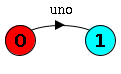
\includegraphics[scale=1]{imagenes/lts-uno}
\end{minipage}
\end{center}

\paragraph{Recursión}
Sirve para modelar repetición de comportamiento
\begin{center}
\begin{minipage}{0.45\textwidth}
\texttt{SWITCH = (on -> off -> SWITCH)}
\end{minipage}
\begin{minipage}{0.415\textwidth}
	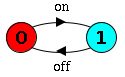
\includegraphics[scale=1]{imagenes/lts-switch}
\end{minipage}
\end{center}

\paragraph{Subprocesos} 
Cuando se debe separar un proceso en subprocesos, se lo puede hacer separandolos con una coma. Cada subproceso declarado solo es válido localmente, es decir, pertenecen a la definición del proceso original y no pueden ser usados por otros.
\begin{center}
\begin{minipage}{0.25\textwidth}
\texttt{SWITCH = OFF,}

\texttt{OFF    = (on -> ON),}

\texttt{ON     = (off -> OFF).}

\end{minipage}
\begin{minipage}{0.25\textwidth}
	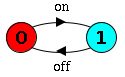
\includegraphics[scale=1]{imagenes/lts-switch}
\end{minipage}
\end{center}

\paragraph{Alternativa} 
Si \texttt{x} e \texttt{y} son acciones entonces \texttt{(x -> P | y -> Q)} describe un proceso que inicialmente es capaz de interacturar a travéz de las acciones \texttt{x} ó \texttt{y}. 
\begin{center}
\begin{minipage}{0.55\textwidth}
\texttt{GIRO = (izquierda -> GIRO | derecha-> STOP).}
\end{minipage}

\vspace*{0.25cm}
\begin{minipage}{0.5\textwidth}
	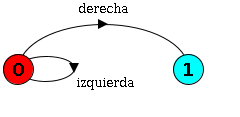
\includegraphics[scale=0.75]{imagenes/lts-giro}
\end{minipage}
\end{center}

\paragraph{Elección no deterministica}
El proceso \texttt{(x -> P | x -> Q)} describe una elección no determinística entre \texttt{P} ó \texttt{Q}.
\begin{center}
\begin{minipage}{0.55\textwidth}
\texttt{MONEDA = (tirar -> CARA | tirar -> SECAS),}

\texttt{CARA = (cara -> MONEDA),}

\texttt{SECAS = (secas -> MONEDA).}
\end{minipage}

\vspace*{0.25cm}
\begin{minipage}{0.5\textwidth}
	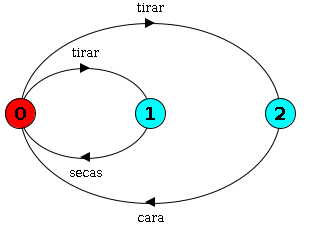
\includegraphics[scale=0.75]{imagenes/lts-moneda}
\end{minipage}
\end{center}
\paragraph{Procesos y acciones indexados:} Nos permiten modelar procesos y acciones que pueden tomar múltiples valores. Los indices siempre tienen un rango finito.

\begin{verbatim}
BUFF = (in[i:0..3] -> out[i] -> BUFF)
\end{verbatim}

\paragraph{Declaración de constantes y rangos:} 
Definimos constantes que pueden ser usadas en cualquier lugar del modelo. Para valores únicos usamos \texttt{CONST} y para rangos \texttt{RANGE}.
\begin{verbatim}
CONST N = 1
RANGE T = 0..N
RANGE R = 0..2*N

SUM = (in[a: T][b:T] -> TOTAL[a + b]),
TOTAL[s:R] = (out[s] -> SUM)
\end{verbatim}

\paragraph{Parámetros de procesos}
Se pueden describir procesos de manera general y pasarle como parámetro una constante inicializada en algún valor para modelar una instancia particular.
El siguiente FSP genera un LTS para un buffer de tres elementos.
\begin{verbatim}
BUFF(N=3) = (in[i: 0..N] -> out[i] -> BUFF).
\end{verbatim}

\paragraph{Guardas}
Se pueden definir acciones de manera condicional, dependiendo del estado actual de una máquina. Usamos guardas booleanas \texttt{when(B) x -> P} para indicar que una acción particular \texttt{x} puede ser elegida si solo si la guarda \texttt{B} es satisfecha.

\begin{verbatim}
COUNT(N=3) = COUNT[0],
COUNT[i:0..N] = (
    when(i < N) inc -> COUNT[i+1] |
    when(i > 0) dec -> COUNT[i-1]
).
\end{verbatim}

\paragraph{Alfabetos}
En LTS tenemos un operador de extensión de alfabeto que extiende el alfabeto implicito de un LTS con las etiquetas deseadas:

\begin{verbatim}
WRITER = (write[1] -> write[3] -> WRITER) + {writer[0..3]}.
\end{verbatim}

\paragraph{Procesos compuestos}
Si \texttt{P} y \texttt{Q} son procesos entonces \texttt{(P||Q)} representa la ejecución concurrente de \texttt{P} y \texttt{Q}.

\begin{verbatim}
ITCH = (sratch -> STOP).
CONVERSE = (think -> talk -> STOP).

||CONVERSE_ITCH = (ITCH || CONVERSE).
\end{verbatim}

\paragraph{Relabeling}
Se aplica a procesos para cambiar el nombre de las etiquetas de acciones. La forma general es \texttt{/\{ nuevaEtiqueta\_1/viejaEtiqueta\_1, ..., nuevaEtiqueta\_n/viejaEtiqueta\_n \}}

\begin{verbatim}
CLIENT = (call -> wait -> continue -> CLIENTE).

SERVER = (request -> service -> replay -> SERVER).

|| CLIENT_SERVER = (CLIENT || SERVER) /{call/request, reply/wait}.
\end{verbatim}

\begin{center}
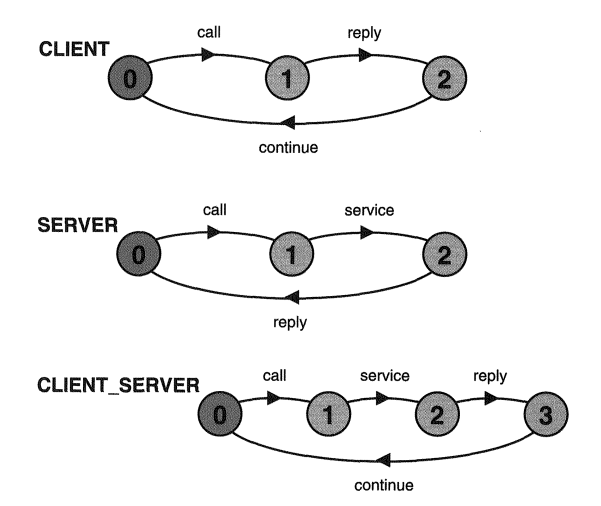
\includegraphics[scale=0.5]{imagenes/lts-clientServer}
\end{center}
\paragraph{Etiquetado de procesos}
Si \texttt{P} es un proceso, entonces \texttt{a:P} prefija, a cada etiqueta del alfabeto de \texttt{P}, la etiqueta \texttt{a}

\begin{verbatim}
|| TWO_SWITCH = (a:SWITCH || b::SWITCH)
\end{verbatim}
\begin{center}
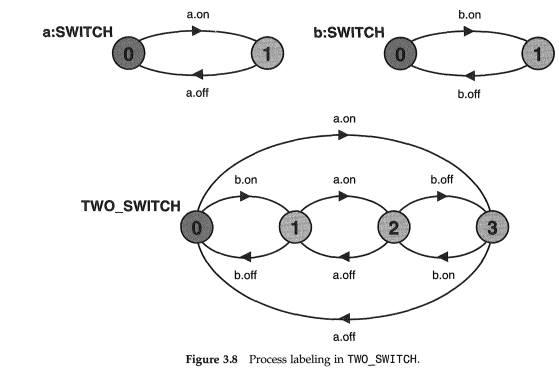
\includegraphics[scale=0.5]{imagenes/lts-dosSwitches}
\end{center}

\paragraph{Generación de etiquetas dentro procesos}
Si \texttt{P} es un proceso, entonces \texttt{{a\_1,...,a\_n}::P} remplaza cada acción \texttt{n} de \texttt{P} por las etiquetas \texttt{a\_1.n,...,a\_x.n}. 

\begin{verbatim}
RESOURCE = (aquire -> release -> RESOURCE).
USER = (aquire -> use -> release -> USER).

|| RESOURCE_SHARE = (a:USER || b:USER || {a,b} :: RESOURCE)
\end{verbatim}
\begin{center}
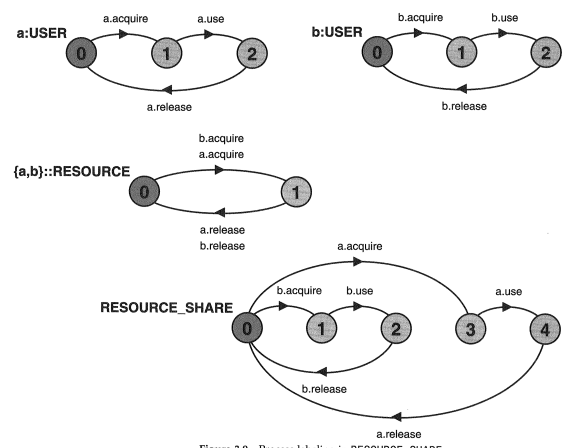
\includegraphics[scale=0.5]{imagenes/lts-resourceShare}
\end{center}

Otra forma de escribir esto es:
\begin{verbatim}
|| SWITCHES(N=3) = ({a,b}:SWITCH)
\end{verbatim}

\paragraph{Ocultamiento de etiquetas}
Cuando se aplica \texttt{$\backslash$\{a1,a2\}} en un proceso \texttt{P}, oculta las etiquetas mencionadas en ese conjunto y convierte las transiciones por estas etiquetas a transiciones por $\tau$.

Cuando se aplica \texttt{@\{a1,a2\}} en un proceso \texttt{P}, oculta las etiquetas no mencionadas en ese conjunto y convierte las transiciones por 
esas etiquetas a transiciones por $\tau$.

Esta definición:
\begin{verbatim}
USER = (aquire -> use -> release -> USER)
    @{aquire, release}.
\end{verbatim}
y esta:
\begin{verbatim}
USER = (aquire -> use -> release -> USER)
    \{use}.
\end{verbatim}
son equivalentes y generan:
\begin{center}
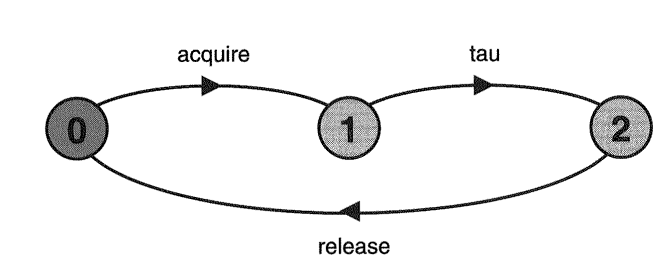
\includegraphics[scale=0.5]{imagenes/lts-user}
\end{center}

\paragraph{For all keyword}
Para cada valor de un rango genera tantas etiquetas / procesos:
\paragraph{Ejemplo:}
\begin{verbatim}
const N = 3
Philosopher = (think -> sit -> left.get -> right.get ->
               eat -> left.put -> right.put -> stand -> Philosopher).
Fork = (get -> put -> Fork).
||DP = (forall [i:0..N] (phil[i]:Philosopher ||
        {phil[i].left,phil[(i+1)%(N+1)].right}::Fork )).
\end{verbatim}

Para correr los tests de progress siempre se asume \textbf{fairness}, esto es que hay equiprobabilidad al momento de transicionar no-deterministicamente por las etiquetas.

\newpage
\section{Verificación de propiedades}

\paragraph{Chequeo exhaustivo:} Se compone el modelo con un proceso de testeo que simula una situación y compara los resultados del modelo con los resultados esperados. Si éste, no responde correctamente el proceso termina en error.

Si, al componer el test con el modelo, hay alguna traza que termina en error entonces ocurrieron alguna de estas dos cosas:

\begin{itemize}
\item El test no modela la propiedad deseada y hay que modificarlo.
\item El modelo no cumple con la propiedad deseada y hay que modificarlo.
\end{itemize}

En LTS tenemos la palabra reservada \texttt{property}, para indicar que un proceso es un propiedad y debe ser completo. Agrega una transición desde cada estado a un estado de error por cada etiqueta no usada desde el mismo.

\subsection{Propiedades de safety}
Son las propiedades que nos aseguran que \textit{nunca suceden cosas malas}. Por ejemplo:
\begin{itemize}
\item No hay deadlock
\item No hay exclusión mutua
\item Siempre se preserva el invariante
\end{itemize}

Un sistema \textbf{satisface} una propiedad de este tipo si no existe ninguna traza en donde lo malo sucede. Si la \textbf{viola}, entonces, podemos mostrar una traza finita en la que esto sucede. 

\subsubsection{Property}
Una \texttt{property} es una FSP completo que describe algo que debe pasar y que si no pasa va a \texttt{ERROR} o a \texttt{STOP}.

En todos sus estados todas las acciones del alfabeto están habilitadas. Todas aquellas que no fueron explícitamente declaradas, van a \texttt{ERROR}.


\begin{verbatim}
property SAFE_ACTUATOR = (command -> respond -> SAFE_ACTUATOR).
\end{verbatim}

\begin{center}
	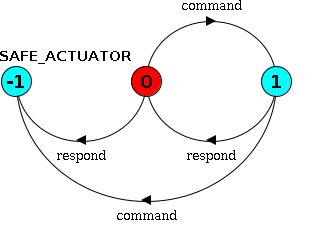
\includegraphics[scale=0.5]{imagenes/lts-safeActuator}
\end{center}


Si, la composición de una \texttt{property} con un sistema, no genera un error o nunca se detiene entonces ese sistema cumple con la propiedad. Llamamos al \textbf{automáta observador} del sistema $A$ al FSP generado con \texttt{property} que describe una propiedad que debe ser cumplida por $A$.

\paragraph{Propiedades}
\begin{itemize}
\item Si $S$ satisface una propiedad safety $P$ entonces $S||T$ también satisface $P$.
\item Si $P$ es un automáta observador y \texttt{ERROR} no es alcanzable en $S||P$, entonces \texttt{ERROR} tampoco es alcanzable en $(S||P)||Q$, cualquiera sea $Q$? (\red{No queda claro})

\end{itemize}

\subsection{Propiedades de Liveness}
Una propiedad de liveness asegura que \textit{algo bueno va a pasar en algún momento}. Un sistema, no cumple una propiedad de este tipo si existe una traza en donde nunca sucede lo bueno.

Para poder garantizar propiedades de liveness deben realizarse algunas suposiciones:

\begin{itemize}
\item \textbf{Weak Fairness:} Si a partir de un instante, una acción está habilitada continuamente, entonces no puede ser ignorada.
\item \textbf{Fair Choice:} Si una elección sobre un conjunto de transiciones es ejecutada infinita veces, entonces cada transición del conjunto será ejecutada infinitas veces.
\end{itemize}

\paragraph{Propiedad:} Si $S$ satisface una propiedad de liveness $P$ entonces $S||T$ también satisface $P$.

\subsubsection{Progress}
Una propiedad de progress es una clase particular de liveness. Indica que siempre debe ser posible (eventualmente) ejecutar una o más acciones.

En LTS tenemos la palabra clave \texttt{property} para definir este tipo de propiedades. Una vez compilado los LTS, debemos correr un \textit{progress check} para verificar que no sean violadas.

\begin{verbatim}
    COIN =(toss->heads->COIN |toss->tails->COIN).
    
    progress HEADS = {heads}.
    progress TAILS = {tails}.
\end{verbatim}

 \paragraph{Conjunto terminal de estados:} Conjunto en donde cada estado es alcanzable desde cualquier otro del conjunto y no existen transiciones de un estado del conjunto a un estado fuera del conjunto.
 
 Una propiedad de progreso se viola si es posible encontrar un conjunto terminal en el que ninguna de las acciones de la propiedad está en el conjunto terminal.
\begin{verbatim}
property USER = (aquire -> use -> release -> USER)
\end{verbatim}

\subsection{Bisimulación}
La  bisimulación es una relación de equivalencia (reflexiva, transitiva y simétrica). Separa los autómatas en clases que no dependen de su cantidad de estados y estructura sino por comportamiento.

La idea, es que dos autómatas $P$ y $Q$ son bisimilares si para cada uno de los estados de $P$, existe un estado equivalente en $Q$. Osea que tanto en $P$ como en $Q$, existen estados que soportan las mismas etiquetas y, además, cualquier estado que acción que realicemos lleve a otro par de estados equivalentes.

\begin{definicion}{Bisimulación fuerte (Strong Bisimilation)}
Sea $\mathcal{P}$ el universo de todos los LTS. Una relación binaria $\mathcal{R}\subseteq\mathcal{P}\times\mathcal{P}$ es una bimisimulación fuerte si y solo si para todo par $(P,Q)\in\mathcal{R}$ vale que para cada acción $a\in Act\cup\{\tau\}$:
\begin{itemize}
\item $(P\overset{a}{\longrightarrow} P') \Rightarrow (\exists Q'$ tal que $Q\overset{a}{\longrightarrow}Q' \land (P', Q')\in\mathcal{R}$ y
\item $(Q\overset{a}{\longrightarrow} Q') \Rightarrow (\exists P'$ tal que $P\overset{a}{\longrightarrow}P' \land (P', Q')\in\mathcal{R}$
\end{itemize}
\end{definicion}

\begin{definicion}{Bisimilaridad fuerte (Strong bisimilarity)}
Dos LTS $P,Q \in \mathcal{P}$ son fuertemente bisimilares $(P \sim Q)$ sii $\exists$ una bisimulación fuerte R tal que $(P,Q) \in R$.

$$\sim  = \cup \{R | R \text{ es una bisimulación fuerte }\}$$

\end{definicion}

\begin{definicion}{Simulación fuerte}
Sea $\mathcal{P}$ el universo de todos los LTS. Una relación binaria $R\subseteq \mathcal{P}\times \mathcal{P}$ es una simulación fuerte si y solo si:
\begin{align*}
(P,Q)\in R \Rightarrow (\forall~&a\in \Sigma\cup\{\tau\}
\\ &((P\overset{a}{\to} P') \Rightarrow (\exists Q' \text{ tal que } Q \overset{a}{\to} Q'~\land~(P',Q')\in R))
)
\end{align*} 
\end{definicion}

\begin{definicion}{Bisimulación débil}
Sea $\mathcal{P}$ el universo de todos los LTS. Una relación binaria $R\subseteq \mathcal{P}\times \mathcal{P}$ es una bisimulación débil sii:
$$(P,Q)\in R \Rightarrow \left(\forall~a\in\Sigma\cup\{\tau\}
\begin{tabular}{c}
    $((P\overset{a}{\to} P') \Rightarrow (\exists Q'$ tal que $Q \overset{a}{\Rightarrow} Q'~\land~(P',Q')\in R))$  \\ $\land$ \\
    $((Q\overset{a}{\to} Q') \Rightarrow (\exists P'$ tal que $P \overset{a}{\Rightarrow} P'~\land~(P',Q')\in R))$ \\
\end{tabular}
\right)$$

Donde: 
$$\overset{a}{\Rightarrow} = \left \{
\begin{tabular}{c c}
    $(\overset{\tau}{\to})^* \circ \overset{a}{\to} \circ(\overset{\tau}{\to})^*$ & si a $\neq \tau$ \\
    $(\overset{\tau}{\to})^*$ & si a = $\tau$ \\ 
\end{tabular}
\right.$$

\end{definicion}

\begin{definicion}{Bimisilaridad débil}
Dos LTS $P,Q \in \mathcal{P}$ son débilmente bisimilares $(P \approx Q)$ sii $\exists$ una bisimulación débil R tal que $(P,Q) \in R$.

\begin{center}
$\approx = \cup \{R | R$ es una bisimulación débil$\}$
\end{center}
\end{definicion}
\subsubsection{El juego de la bisimilaridad}
\paragraph{Juego de la Bisimilaridad fuerte}
Sean $P$ y $Q$ dos LTS, el juego consiste en un \textbf{atacante} y un \textbf{defensor}. El atacante intenta demostrar que $P$ y $Q$ no son bisimilares y, el defensor, que lo son.

En cada ronda, los jugadores cambian la configuración del juego cambiando el estado de uno de los autómata de la siguiente manera:
\begin{itemize}
    \item El atacante elije uno de los procesos en la configuración corriente y hace una movida por alguna transición con etiqueta $a$ en alguno de los procesos.
    \item El defensor debe responder haciendo una movida por una transición etiquetada con $a$ en el  proceso.
\end{itemize}

Si el juego es infinito, entonces el defensor gana y $P$ y $Q$ son bisimilares. Si, en algún momento, el defensor no puede realizar la acción que realiza el atacante entonces el juego termina, gana el atacante y $P$ y $Q$ no son bisimilares.

Si son bisimilares, entonces hay que dar la relación de bisimilaridad. Para esto, hay que conseguir todos los pares de estados que pertenecen a ella, osea, hay que conseguir todos los pares $(p,q)\in P\times Q$ que pueden ser alcanzados por una etiqueta.

\paragraph{Juego de la Bisimilaridad débil:} Idem anterior, pero ahora el defensor puede moverse por $\Rightarrow$ y, el atacante, por a lo sumo, un $\tau$ \red{(o no, la verdad esto no queda claro. Los tipos nunca no nos supieron decir asi que, si alguien se entera, por favor, avise)}.

\newpage
\part{Lógica Temporal Lineal}
\section{Estructuras de Kripke}
\begin{definicion}{Estructura de Kripke}
Una \textbf{estructura de Kripke} es un par $(W,R)$ tal que:
\begin{itemize}
\item $W$ es un conjunto de nodos,
\item $R$ es una relación binaria sobre $W$ ($R\subseteq W\times W$).
\end{itemize}

O sea que es \textbf{es un grafo}. 
\end{definicion}

\begin{definicion}{Función de evaluación}
Una \textbf{función de evaluación} $v:Pr\times W \to \{T,F\}$ asigna a cada proposición un valor de verdad en cada estado del posible.
\end{definicion}

Las estructuras de Kripke, junto con una función de evaluación nos permite representar un programa en base a las propiedades que se deben cumplir en cada uno de sus estados. Cada estado es un nodo y se une con flechas a todos los estados a los que puede pasar el programa desde ese estado. La función de evaluación, nos indica que propocisiones son validad en cada momento de la ejecución.

\paragraph{Ejemplo de Modelo con Krikpe}
\begin{center}
    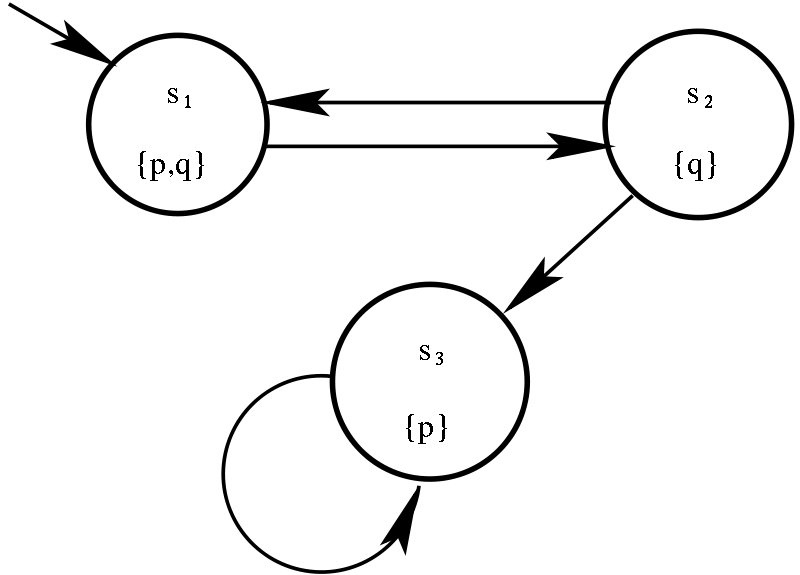
\includegraphics[scale=0.3]{imagenes/kripke.png}
\end{center}

El kripke representa un programa de tres estados $W=\{s_1,s_2,s_3\}$ en el que pueden valer dos proposiciones $p$ y $q$. En cada estados, marcamos cuales de ellas vale entre llaves. Osea que en $s_1$ valen las dos, en $s_2$ vales solo $q$ y en $s_3$ solo $p$.

\begin{definicion}{Traza}
Una traza de una estructura de Kripke son una secuencia infinita de estados $\sigma = \{\sigma_0,\sigma_1,\dots\}$ que representa la ejecución de un programa. $\sigma_i$ representa el estado al que llegó el programa en el $i$-ésimo paso.
\end{definicion}

\newpage
\section{Lógica temporal lineal (LTL)}
\begin{itemize}
\item Variables proposicionales: $p,~q,~r,\dots$
\item Conectivos lógicos clásicos
\begin{multicols}{2}
\begin{itemize}
\item Conjunción $(p \land q)$
\item Disyunción $(p \lor q)$
\item Negación $(\lnot p)$
\item Implicación $(p \implies q)$
\end{itemize}
\end{multicols}
\item Operadores modales:
\begin{multicols}{2}
\begin{itemize}
\item Siempre ($\square p$ ó G$p$)
\item Eventualmente ($\Diamond p$ ó F$p$)
\item En el próximo paso (X$p$)
\item Hasta que ($p$ U $q$)
\end{itemize}
\end{multicols}
\end{itemize}

Nos va a servir para hablar sobre propiedades de alguna ejecución de un programa, es decir, sobre propiedades de alguna de las trazas de un modelo de Kripke.


\subsection{Semántica}
Dada una estructura de Kripke $(W,R)$, una función de evaluación $v$ y $\sigma$ una traza del Kripke decimos que un estado $w$ satisface la formula $\psi$ si $\psi$ es verdadera en ese estado. Sea $p$ y $q$ proposiciones de la lógica modal, entonces:
\begin{itemize}
    \item $\sigma[i] \vDash p$ si y solo si $v(p,\sigma[i])$
    \item $\sigma[i] \vDash \text{X}p$ si y solo si $\sigma[i+1]\vDash p$
    \item $\sigma[i] \vDash \lozenge p$ si y solo si $(\exists~j: i \leq j)~\sigma[j] \vDash p$
    \item $\sigma[i] \vDash \square p$  si y solo si $(\forall~j: i \leq j)~\sigma[j] \vDash p$
    \item $\sigma[i] \vDash p \text{ U } q$ si y solo si $(\exists~k: i \leq k) (\sigma[k] \vDash q ~\wedge~ ((\forall~j: i \leq j < k)~\sigma[j] \vDash p))$
\end{itemize}

Decimos que una traza $\sigma$ satisface una formula $\psi$ ($\sigma\vDash\psi$) si y solo si $\sigma[0] \vDash \psi$.


\newpage
\section{Verificación de programas y model checking}
Decimos que un modelo $M$ (Kripke) satisface un fórmula $\psi$ de LTL si y solo si para toda traza $\sigma$ de $M$, vale $\sigma\vDash\psi$.

\subsection{Autómata de buchi}
\begin{definicion}{Autómata de Büchi}
Son autómatas de estados finitos que reconocen lenguajes de palabras infinitas. Solo aceptan una cadena si pasa infinitas veces por uno o más estados de aceptación.

Los vamos a usar para representar conjuntos de trazas de un sistema que cumplan ciertas propiedades. 
\end{definicion}

\begin{figure}[h]
\centering
	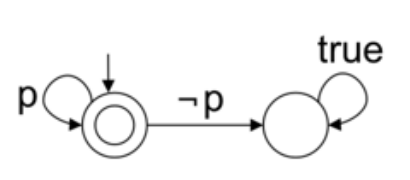
\includegraphics[scale=0.5]{imagenes/buchi-siempre-p}
	\caption{Autómata de buchi para la fórmula $\square p$. Se mantiene en un estado de aceptación mientras valga $p$. En el primer momento que no lo hace, va al segundo estado y se queda ciclando en el mismo (sin importar el valor actual de $p$).}
\end{figure}

\subsection{Método de verificación}
Para comprobar que una fórmula $P$ de la lógica temporal es satisfecha por una estructura de Kripke $M$ debemos hacer lo siguiente:
\begin{enumerate}
    \item Convertir la formula $\lnot P$  en un autómata de Büchi $AP$ (No dijeron como hacer esto, hacerlo por intuición y rogar que este bien).
    \item Convertir el Kripke $M$ en un autómata de Büchi $AM$. Todos los estados del autómata generado son de aceptación.
    \item Componer $AM$ con $AP$ (los autómatas de los dos pasos anteriores)
    \item Verificar si el lenguaje que acepta la composición es vació. Debemos buscar un ciclo que contenga un estado de aceptación y sea alcanzable desde el estado inicial.
    \begin{itemize}
    	\item Si el lenguaje es vacío entonces se cumple $P$.
    	\item Si no lo es, existe una traza en $M$ que cumple la negación de $P$ y funciona como contra ejemplo.
    \end{itemize}
\end{enumerate}
\paragraph{Ejemplo:}
\begin{center}
    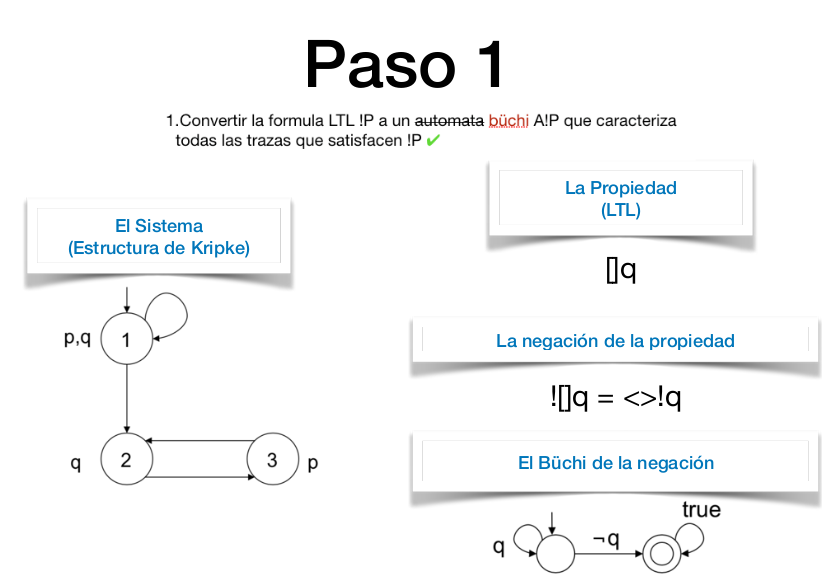
\includegraphics[scale=0.375]{imagenes/paso1.png}
    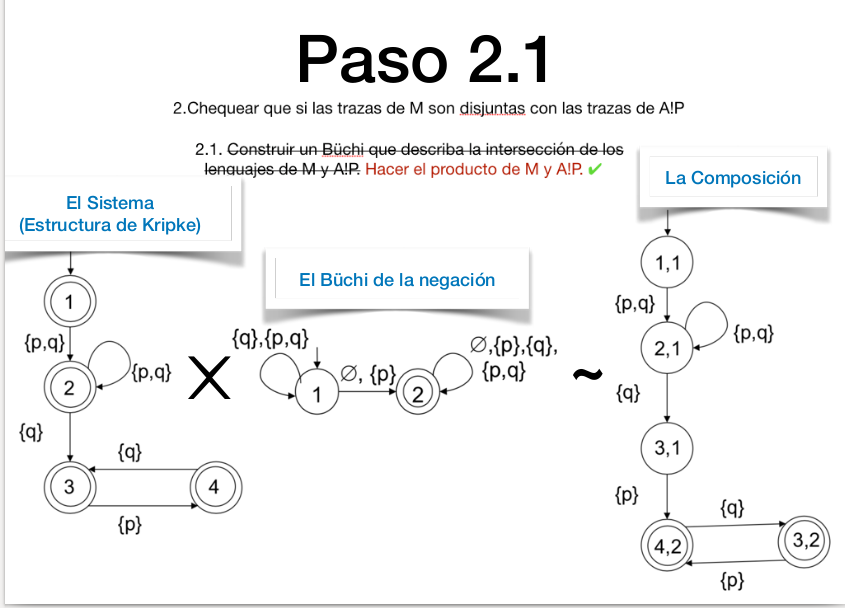
\includegraphics[scale=0.375]{imagenes/paso2.png}
    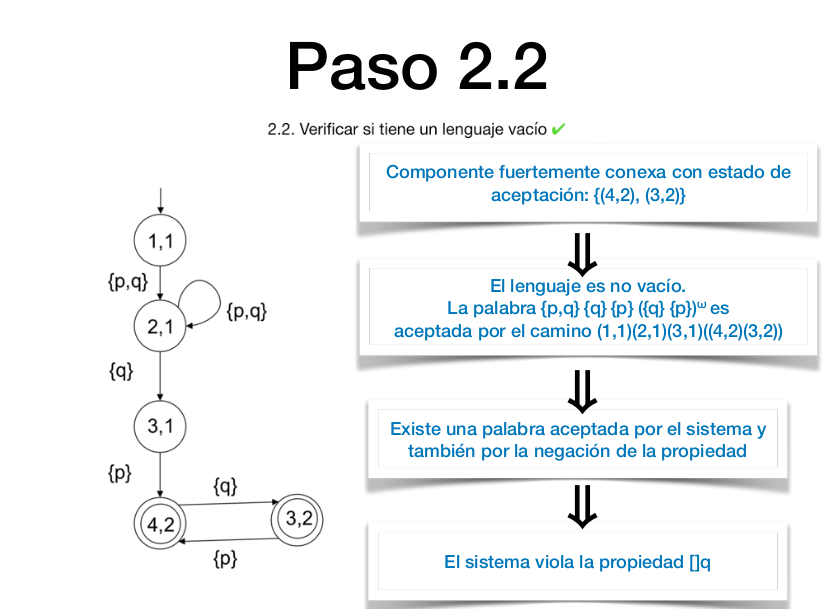
\includegraphics[scale=0.375]{imagenes/paso2-2.png}
\end{center}

\newpage
\part{Lógica Computacional Árborea (Computacional Tree Lógic, CTL)}
\section{Sintaxis y semantica}
A diferencia de LTL, que se concentra en una única traza, nos va a permitir describir propiedades sobre la totalidad de las trazas de un sistema. Dejamos de verlas como caminos disconexos para pasar a representarlas como arboles de ejecución.

\begin{figure}[h]
\centering
	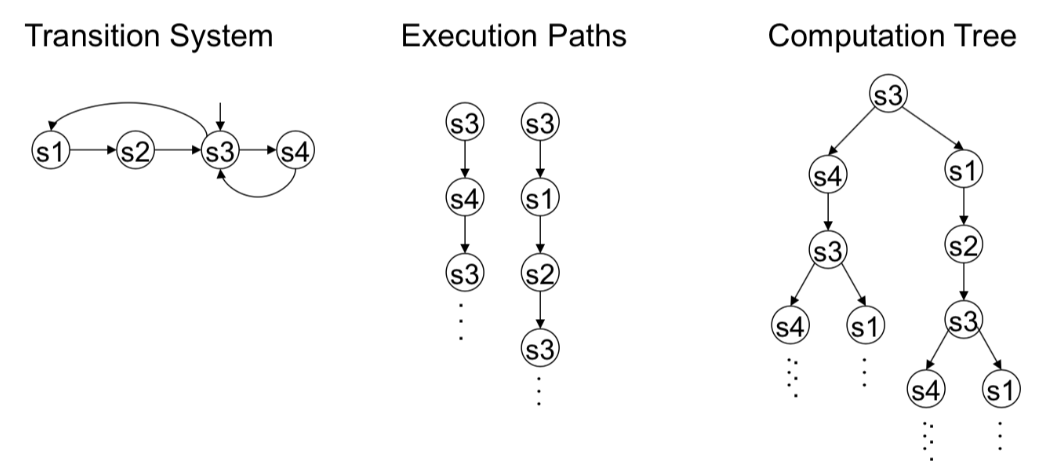
\includegraphics[scale=0.25]{imagenes/ctl-ltl-comparison}
\end{figure}

Agrega las cuantificaciones A y E a los operadores modales, lo que permite, asertar cosas sobre todos los caminos que derivan de un nodo:
\begin{itemize}
\item A: Para todo camino
\item E: Existe un camino
\end{itemize}

\begin{definicion}{Función de evaluación L}
Dado un conjunto de proposiciones atómicas $AP$ y una estructura de Kripke $M=(W,R)$ sobre $AP$, la función $L:W\to 2^{AP}$ toma un estado de $M$ y devuelve el conjunto de proposiciones que valen en ese estado (la imagen de la función es el conjunto de parte de AP).
\end{definicion}
\subsection{Semántica}
Dado un árbol de cómputo infinito satisface una formula si su raíz $s_0$ lo hace. Sean $p$ y $q$ dos fórmulas de CTL:
\begin{itemize}
    \item $s \vDash p$ si y solo si $v(p,s)$
    \item $s_0 \vDash \text{EX } p$ si y solo si existe un camino $S =\{s_0,\dots\}$ tal que $S[1]\vDash p$
    \item $s_0 \vDash \text{AX } p$ si y solo si para todo camino $S$ de la forma $\{s_0,\dots\}$ vale que $S[1]\vDash p$
    \item $s_0 \vDash \text{EG } p$ si y solo si existe un camino $S =\{s_0,\dots\}$ en el que siempre vale $p$ .
    \item $s_0 \vDash \text{AG } p$ si y solo si para todo camino $S$ de la forma $\{s_0,\dots\}$ siempre vale $p$ ($\forall~i\geq 0$ vale $S[i] \vDash p$).
    \item $s_0 \vDash \text{EF } p$ si y solo si existe un camino $S=\{s_0,...\}$ en el que, en algún momento, vale $p$ ($\exists~i\geq 0$ tal que  $S[i] \vDash p$).
    \item $s[0] \vDash \text{AF } p$ si y solo si para todo camino  $S$ de la forma $\{s_0,\dots\}$ vale, en algún momento, $p$ ($\exists~i\geq 0$ tal que  $S[i] \vDash p$).
    \item $s_0 \vDash p \text{ EU } q$ si y solo si existe un camino $S =\{s_0,\dots\}$ tal que \\\hspace*{1cm} $(\exists i\geq 0)~(S[i] \vDash q~\land~(\forall~ 0\leq j\leq i)~S[j]\vDash p))$.
    \item $s_0 \vDash p \text{ AU } q$ si y solo si para todo camino  $S$ de la forma $\{s_0,\dots\}$ vale que\\\hspace*{1cm} $(\exists i\geq 0)~(S[i] \vDash q~\land~(\forall~ 0\leq j\leq i)~S[j]\vDash p))$.
\end{itemize}

\newpage
\section{Verificación de propiedades y Model Checking}
Dado una estructura de Kripke, deseamos determinar si su árbol de cómputo cumple con una fórmula $P$ de CTL. Para esto, debemos representar las fórmulas como conjuntos de estados

\subsection{Fórmulas como conjuntos característicos}
\begin{definicion}{Conjunto característico}
Dados un modelo $M = \langle(W,R), v\rangle$ sobre un conjunto de proposiciones átomicas ($AP$) y una fórmula de CTL $\phi$. El conjunto característico $\charset{\phi}{M}$ de $\phi$ sobre $M$ es el conjunto de estados en el $\phi$ es verdadera.
\end{definicion}


\paragraph{Semántica de CTL vista como conjuntos característicos}
\begin{itemize}
\item $\charset{a}{M} = \{s \in W ~|~ v(s,a) = \text{True} \}$ para $a\in AP$
\item $\charset{\lnot\phi}{M} = W - \charset{\phi}{M}$
\item $\charset{\phi_1\lor\phi_2}{M} = \charset{\phi_1}{M} \cup \charset{\phi_2}{M}$
\item $\charset{\phi_1\land\phi_2}{M} = \charset{\phi_1}{M} \cap \charset{\phi_2}{M}$
\item $\charset{\text{EX }\phi}{M} = \{s\in W~|~\exists~t\in$ Post($s$) tal que $t\in\charset{\phi}{M}\} = \{ s \in W~|~$ Post($s) \cap \charset{\phi}{M} \neq\emptyset\}$.
\item $\charset{\text{EG }\phi}{M} = \{s\in W~|$ existe un camino $S=\{s,\dots\}$ tal que para todo estado $S[i]$ con $i\geq 0$, $S[i]\in\charset{\phi}{M} \}$

Es el mayor conjunto $T\subseteq W$ que satisface:
\begin{enumerate}
\item $T\subseteq\charset{\phi}{M}$ (\textit{son estados que satisfacen $\phi$}) y
\item $s\in T \implies$ Post$(s)\cap T \neq\emptyset$ (\textit{si un estado de $T$ tiene un estado siguiente, entonces ese estado también está en $T$}).
\end{enumerate}

\item $\charset{\phi_1 \text{ EU }\phi_2}{M} = \{s\in W~|$ existe un camino $S=\{s,\dots\}$ tal que para algún estado $S[i]$ con $i\geq 0$, $S[i]\in\charset{\phi_2}{M}$ y para todo $k < i$, $S[k]\in\charset{\phi_1}{M} \}$

Es el mínimo conjunto $T\subseteq W$ que satisface las siguientes fórmulas:
\begin{enumerate}
	\item $\charset{\phi_2}{M}\subseteq T$ (\textit{todos los estados que satisfacen $\phi_2$ están en $T$}) y
	\item $(s\in\charset{\phi_1}{M}~\land$ Post$(s)\cap T \neq\emptyset) \implies s\in T$ (\textit{si un estado de $T$ tiene un estado anterior que satisface $\phi_1$ entonces, ese estado, está en $T$})
\end{enumerate}
\end{itemize}

\red{El resto de las caracterizaciones faltan en la teóricas, pero acá van:}
\begin{itemize}
\item $\charset{\text{AX }\phi}{M} = \{s\in W~|~\forall~t\in$ Post($s$) tal que $t\in\charset{\phi}{M}\} = \{ s \in W~|~$ Post($s) \subseteq \charset{\phi}{M}\}$.
\item $\charset{\text{AG }\phi}{M} = \{s\in W~|$ para todo camino $S=\{s,\dots\}$ vale que $\forall~i\geq 0,~S[i]\in\charset{\phi}{M} \}$

Es el mayor conjunto $T\subseteq W$ que satisface $T \subseteq \{ s \in\charset{\phi}{M}~|$ Post$(s) \subseteq T \}$.

\item $\charset{\phi_1 \text{ AU }\phi_2}{M} = \{s\in W~|$ para todo camino $S=\{s,\dots\}$ vale que para algún estado $S[i]$ con $i\geq 0$, $S[i]\in\charset{\phi_2}{M}$ y para todo $k < i$, $S[k]\in\charset{\phi_1}{M} \}$

Es el mínimo conjunto $T\subseteq W$ que satisface 
\begin{enumerate}
\item $\charset{\phi_2}{M} \subseteq T$ y
\item $\{s\in\charset{\phi_1}{M} ~|~$ Post$(s)\subseteq T\} \subseteq T$
\end{enumerate}
\end{itemize}


Decimos que un modelo $M$ satisface $\phi$ ($M\vDash \phi$) si y solo si la raíz $s_0$ de su árbol computacional la satisface ($s_0 \in\charset{\phi}{M}$).

\subsection{Algoritmo de punto fijo}
\begin{definicion}{Punto fijo}
Dada una función $f:D\to D$, $x\in D$ es un punto fijo de $f$, si y solo sí $f(x)=x$
\end{definicion}

\newpage
\part{Apéndices}
\appendix
\section{Diagramas de bloque}
Son usados para modelar interacción entre procesos. Cada proceso es representado como un bloque con círculos en su perímetro que indican las acciones visibles desde el entorno.
\begin{figure}[h]
\centering
	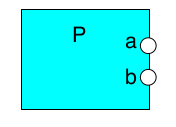
\includegraphics[scale=0.5]{imagenes/bloque_proceso}
	\caption{Proceso P con alfabeto \{a,b\}}
\end{figure}

La composición en paralelo de dos procesos se representa uniendo dos bloques con líneas entre las acciones que deben sincronizar (y si se necesita un renombre, sobre las líneas marcar el nombre de la acción).

\begin{figure}[h]
\centering
	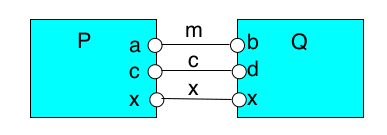
\includegraphics[scale=0.5]{imagenes/bloque_composicion}
	\caption{Compocisión de los procesos P y Q con renombre de acciones (P$||$Q) /\{m/a, m/b, c/d\}}
\end{figure}

Y el proceso $||$S que solo muestra ciertas acciones de la interacción, se representa encerrando la figura anterior dentro de otro proceso:

\begin{figure}[h]
\centering
	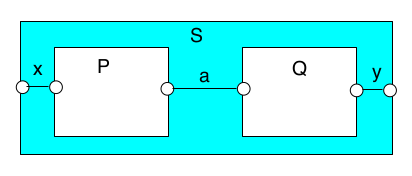
\includegraphics[scale=0.5]{imagenes/bloque-proceso-compuesto}
	\caption{Proceso S conseguido a partir de la compocisión de los procesos ConversationsP y Q: $||$S = (P$||$Q) @ \{x,y\}}
\end{figure}


\end{document}



